\section{Beale Function}
\label{sec:beale_function}

Unveiled by Beale in 1958\footnote{
  Beale, E. M. (1958). \enquote{On an Iterative Method for Finding a Local 
  Minimum of a Function of More than One Variable}. 
}, the Beale function is recognized for its multimodal characteristics and 
sharp peaks that define the domain's corners.

\begin{definition}[Beale Function]
  \label{def:beale_function}
  The \emph{Beale Function}, symbolized as \(f: \mathbb{R}^2 \rightarrow 
  \mathbb{R}\), is expressed by the equation:

  \begin{equation}
  \label{eq:beale_function}
    f(x,\,y) = (1.5 - x + xy)^2 + (2.25 - x + xy^2)^2 + (2.625 - x + xy^3)^2
  \end{equation}

  It's evaluated within the domain \(x,\, y \in [-4.5,\,4.5]\).
\end{definition}

The global minimum of the Beale function is found at \(f(3,\,0.5) = 0\).
Both contour and surface plots of the Beale function are depicted in 
\vref{fig:beale_function}.

\begin{figure}[ht!]
  \centering
  \begin{subfigure}[b]{0.45\textwidth}
    \centering
    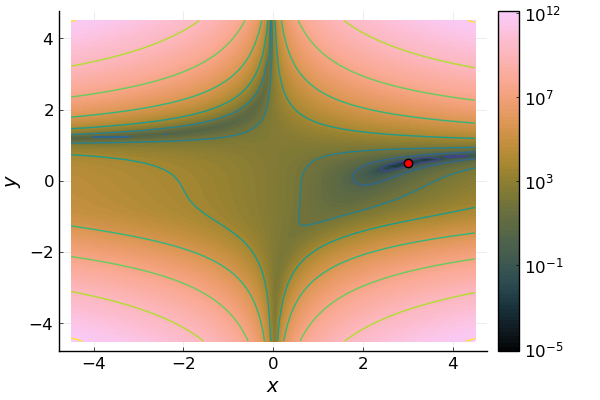
\includegraphics[width=\textwidth]{img/test_functions/beale_contour.png}
    \caption{Contour plot of the Beale Function}
  \end{subfigure}
  \hfill
  \begin{subfigure}[b]{0.45\textwidth}
    \centering
    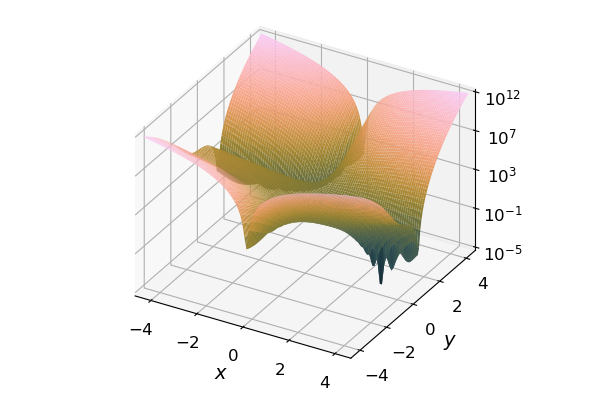
\includegraphics[width=\textwidth]{img/test_functions/beale_surface.png}
    \caption{Surface plot of the Beale Function}
  \end{subfigure}
  \caption{Visual representation of the Beale Function}
  \label{fig:beale_function}
\end{figure}
